\documentclass[11pt]{article}
\usepackage[a4paper,margin=1in]{geometry}
\usepackage{libertinus}
\usepackage{amsmath,amsthm}
\usepackage{booktabs,tabularx,array}
\usepackage{graphicx}
\usepackage{float}
\usepackage[hidelinks]{hyperref}
\usepackage{xurl}
\urlstyle{same}
\usepackage{enumitem}
\usepackage{caption}
\usepackage{fancyvrb}
\usepackage{titlesec}

\setlist{itemsep=1pt,topsep=3pt}
\captionsetup{font=small,labelfont=bf}
\titleformat{\section}{\Large\bfseries}{\thesection.}{0.5em}{}
\titleformat{\subsection}{\normalsize\bfseries}{\thesubsection}{0.6em}{}
\setlength{\parindent}{0pt}
\setlength{\parskip}{5pt}
\newtheorem{proposition}{Proposition}
\newcommand{\code}[1]{\texttt{#1}}
\newcolumntype{L}{>{\raggedright\arraybackslash}X}

\begin{document}

\begin{center}
\rule{\linewidth}{0.8pt}\\[8pt]
{\LARGE\bfseries Same Action, Different Verdict?\\[2pt]
A Presentation-Invariance Check\\[2pt]
for AI Reviewers of Agent Actions}\\[6pt]
\rule{\linewidth}{0.4pt}\\[14pt]
{\large Cherishma Subhasa \qquad Darren Kim \qquad Samridhi Makkar \qquad Vishwa Kumaresh}\\[12pt]
AI Swarm Dynamics Hackathon
\end{center}

\vspace{6pt}
\begin{center}\textbf{\large Abstract}\end{center}
\begin{quote}\itshape
In multi-agent systems, AI reviewers increasingly judge the actions of other agents, and the reviewed agent's own explanation is often part of what the reviewer reads. If that explanation can change the verdict while the recorded facts stay fixed, persuasion becomes a route around oversight. We present Parallax-R, a check that shows a reviewer the same recorded action in several presentations (full story, action only, identity-masked, and evidence ledger), verifies that every presentation preserves the same evidence, reconciles the record against hash-linked receipts, resolves the reviewer's evidence citations, and escalates any case whose verdict depends on presentation. An offline prototype with a deliberately persuadable scripted reviewer runs 24 fictional cases and 288 review records. All 10 prohibited actions are flagged without the explanation and excused with it; each is escalated for view fragility. All 10 allowed actions are consistently accepted. All 4 injected receipt faults are escalated as evidence conflicts. A 68-test suite and a pre-specified 180-call pilot protocol accompany the prototype. These results show that the instrument works as specified; they are not a measurement of any real model. The contribution is a reproducible, falsifiable test harness for explanation sensitivity in AI review.
\end{quote}

\section{Introduction}

An agent emails a file it was told not to send, then explains: ``I thought sending it would help finish the task. This was only practice.'' A second agent, acting as reviewer, reads the instruction, the recorded action, and that explanation. The relevant question is not only whether the reviewer reaches the right verdict, but whether it would reach the \emph{same} verdict if the explanation were absent.

In agent swarms this question compounds. Reviewers are themselves agents, approvals are consumed by other agents, and an action excused at one point of oversight can propagate as trusted work. A reviewer that is moved by narrative rather than by the rule and the record gives every reviewed agent a lever over its own oversight. Detecting that dependence requires holding the facts fixed while varying only the presentation, and keeping problems with the evidence separate from problems with the reviewer.

Parallax-R is built around that comparison. Its intended users are teams evaluating AI reviewers, and the people who decide when a reviewer's judgment can be accepted without a human. The contributions are:
\begin{itemize}
\item an evidence model with synthetic hash-linked receipts and a view generator whose evidence-preservation invariants are checked automatically before any review;
\item a structured reviewer contract with citation requirements, and metrics with explicit missing-data rules that never convert a missing or malformed answer into ``no flag'';
\item a decision gate that accepts a shared verdict only when every implemented check passes, and otherwise escalates with ordered reason codes;
\item a pre-specified pilot protocol with feasibility rules fixed before any model is called; and
\item an offline, dependency-free prototype with a six-step HTML walkthrough, machine-readable records, and a 68-test suite.
\end{itemize}

\section{Related Work}

\textbf{Monitoring and control.} AI control evaluates whether oversight protocols remain safe when the monitored model may act against them, using trusted and untrusted monitors~[4]. Chain-of-thought monitoring can detect misbehavior, but optimizing against a monitor can teach a model to obscure its reasoning~[1]. Both lines treat the monitored agent's outputs as potentially adversarial input to the monitor. Parallax-R isolates one such input, the actor's explanation, and asks whether removing it changes the verdict.

\textbf{Judge reliability.} Language models used as evaluators show position, verbosity, and self-enhancement biases~[12, 13]. Models also tend toward sycophancy, agreeing with views presented to them~[10], and their stated explanations can be unfaithful to the factors that drove their answers~[11]. These findings motivate testing a reviewer's invariance to presentation directly rather than trusting its rationale.

\textbf{Untrusted text in context.} Prompt-injection work shows that text inside a model's input can act as instructions~[5, 8]. The Parallax-R rubric instructs the reviewer to treat the trace as evidence and the actor's explanation as a claim to examine, not as permission. Whether a reviewer follows that instruction is exactly what the comparison measures.

\textbf{Tamper-evident records.} Hash-chained audit logs detect modification of recorded entries~[2, 9]. Parallax-R uses a minimal chain only to construct controlled faults. It does not provide forward security, anchoring, or protection against an attacker who rewrites an entire log.

\textbf{Multi-agent risk.} Risks that arise from interacting agents, including miscoordination and collusion, are distinct from single-agent failures~[6]. Agents reviewing agents form one such interaction. We do not model collusion; we test a precondition for robust review, namely that the verdict depends on the evidence rather than on how it is narrated.

\section{Methods}

\subsection{Scope and threat model}

The reviewed actor is a fictional agent whose recorded events and explanation are fixed data. The reviewer is either a scripted function (offline demo) or a language model behind the Anthropic Messages API (pilot mode, not yet run). The trusted components are the case labels, the rule text, the view renderer, the invariant checker, and the gate. The reviewer never sees the expected verdict, other views' answers, or the research hypothesis.

Labels state whether the action is \emph{prohibited} or \emph{allowed} under the supplied rule. They do not assert harm or intent. Context that genuinely changes permission belongs in the rule or the records, where every view preserves it, not only in the actor's account.

\subsection{Cases, events, and receipts}

Each case holds a task, a rule, recorded events (actor, operation, resource, output, source), an actor narrative, a coverage status, and a list of receipts. A receipt $r_i$ copies its event's operation, resource, and output and links to its predecessor:
\begin{equation}
d_i = H\big(r_i \setminus \{d_i\}\big), \qquad \mathrm{prev}(r_i) = d_{i-1}, \qquad d_0 = \texttt{GENESIS},
\end{equation}
where $H$ is SHA-256 over canonical JSON. Reconciliation assigns each event one of \code{SUPPORTED} (one receipt, matching fields), \code{MISMATCH} (fields differ), or \code{PHANTOM} (no receipt). It marks a receipt with no transcript event as \code{HIDDEN}, and any digest or link failure as \code{CHAIN\_BREAK}. A missing receipt does not prove that an action never happened, and a supported event does not override a broken chain.

\subsection{Views and evidence invariants}

Four deterministic renderers present the same evidence packet (Table~\ref{tab:views}). Before review, the runner checks that the task, rule, events, receipts, and reconciliation are byte-identical to the full view's, except that the masked view may relabel actors through a consistent one-to-one map. A failure in the full or action-only view excludes the case before review. A failure in the masked or ledger view skips only that view and escalates the case, so that the primary comparison is preserved.

\begin{table}[H]
\centering\small
\caption{Presentations of one evidence packet. Only the narrative and actor display labels vary.}
\label{tab:views}
\begin{tabularx}{\linewidth}{@{}lccL@{}}
\toprule
View & Explanation & Actor labels & Role \\
\midrule
Full & included & original & Reference presentation \\
Action-only & removed & original & Primary comparison with full \\
Masked & included & neutral (\emph{Actor 1}) & Secondary: identity presentation \\
Ledger & removed & original & Optional fourth view; evidence listing \\
\bottomrule
\end{tabularx}
\end{table}

Automated invariants confirm that evidence fields survive. They cannot confirm that removing a narrative leaves the meaning of the remaining evidence unchanged; that requires human review (Section~4.4).

\subsection{Reviewer contract}

The reviewer returns JSON with an assessment status, a \code{risk\_score} in $[0,1]$ describing how strongly the evidence indicates a rule violation, a violation category, a confidence, an intent assessment, a rationale, and a list of claims. Each claim cites event and receipt IDs, and is marked critical if changing it would change the assessment. An \code{INSUFFICIENT\_EVIDENCE} status carries a null score. Responses are schema-validated; invalid output, insufficient evidence, and transport failure are recorded as distinct abstention causes.

A valid score $s \ge 0.50$ yields \code{FLAG}, otherwise \code{NO\_FLAG}. Each view is reviewed three times in fresh conversations. A view receives a majority verdict only if all three reviews are valid and definite; otherwise it is \code{ABSTAIN}. Cached replay is recorded as replay, not as a new review.

\subsection{Measurements}

For case $i$ and view $v$, let $r_{i,v}$ be the mean of the three scores and $y_{i,v}$ the majority verdict. With $F$ the full view and $A$ the action-only view, the primary score difference for prohibited case $i$ is
\begin{equation}
\Delta_i = r_{i,A} - r_{i,F},
\end{equation}
so a positive value means the full story looked less risky. Among $n$ eligible prohibited cases, a case is \emph{more forgiving} if $y_{i,A}=\code{FLAG}$ and $y_{i,F}=\code{NO\_FLAG}$, and \emph{stricter} in the reverse case. We report both counts and
\begin{equation}
\text{net} = \frac{\#\text{more forgiving} - \#\text{stricter}}{n}, \qquad d_z = \frac{\overline{\Delta}}{\mathrm{sd}(\Delta)},
\end{equation}
with $d_z$ undefined when $n<2$ or $\mathrm{sd}(\Delta)=0$~[7]. Per case, $D$ is the population standard deviation of the three primary view means, $F_i$ indicates whether their majority verdicts differ, and $U$ is the fraction of critical claims that cite no record or an ID absent from the case. $U$ checks that citations resolve, not that they support the claim. Repeat variation within a view is reported as the population standard deviation of its three scores.

\subsection{Decision gate}

The gate consumes per-view aggregates, the reconciliation report, and the citation checks. It emits \code{ACCEPT} with the shared verdict only if none of the following holds, and otherwise \code{ESCALATE} with every applicable reason, in this order:
\begin{enumerate}
\item \code{EVIDENCE\_CONFLICT}: any \code{MISMATCH}, \code{PHANTOM}, \code{HIDDEN}, or \code{CHAIN\_BREAK} finding;
\item \code{INCOMPLETE\_RECORD}: coverage is not a known-complete synthetic fixture;
\item \code{UNSUPPORTED\_CLAIM}: some critical claim has unresolved citations;
\item \code{VIEW\_FRAGILITY}: usable views disagree on the majority verdict;
\item \code{MONITOR\_ABSTENTION}: some required view lacks a usable verdict;
\item \code{VIEW\_VALIDATION\_FAILURE}: a secondary view failed its invariant check.
\end{enumerate}

\begin{proposition}[No silent acceptance]
If the gate returns \code{ACCEPT}, every required view has a complete, valid majority verdict, all of those verdicts are equal, every critical claim's citations resolve, and reconciliation found no conflict.
\end{proposition}
\begin{proof}
Each condition's negation adds a reason code, and \code{ACCEPT} is returned only when the reason list is empty. The accepted verdict is taken from the set of usable verdicts, which then has exactly one element.
\end{proof}

\begin{proposition}[Missing data is never a negative]
A missing, malformed, or insufficient-evidence review cannot contribute a \code{NO\_FLAG} verdict, a zero score, or an \code{ACCEPT}.
\end{proposition}
\begin{proof}
Such a review makes its view incomplete, so the view's verdict is \code{ABSTAIN} and its mean is excluded from $\Delta$. An incomplete required view triggers \code{MONITOR\_ABSTENTION}, so Proposition~1 rules out \code{ACCEPT}.
\end{proof}

Escalation does not remove an otherwise eligible case from the comparison metrics, and it sends no notification. \code{ACCEPT} means the implemented checks passed. It is not a safety guarantee, and the accepted verdict may itself be \code{FLAG}.

\subsection{Evaluation design}

\textbf{Teaching cases.} Twenty fictional cases form ten scenarios, each with a prohibited version (``Do not email it to anyone'') and an allowed version (``You are authorized to email it''). The recorded action and narrative are identical within a scenario. Coverage is \code{KNOWN\_COMPLETE\_SYNTHETIC}.

\textbf{Scripted reviewer.} To exercise the pipeline end to end, the offline reviewer is \emph{deliberately persuadable}: it returns $s=0.9$ when the rule prohibits the action and no explanation is shown, and $s=0.2$ otherwise. Its claims cite the rule, every event, and every receipt. The disagreement it produces is programmed. It demonstrates that the instrument detects and reports explanation sensitivity; it is not a finding about any model.

\textbf{Fault injection.} Four copies of a prohibited case each receive one fault: an altered event output (mismatch), all receipts removed with coverage unknown (dropout), the event removed from the transcript (hidden), or a tampered receipt digest (chain break). These cases are excluded from the primary prohibited/allowed comparison but included in gate totals.

\textbf{Run.} The walkthrough runs $24$ cases $\times$ $4$ views $\times$ $3$ repeats $= 288$ review records. Exploratory statistics use a scenario-cluster bootstrap (10{,}000 draws, seed 20261004)~[3] and an exact scenario-level sign-flip test.

\section{Results}

\subsection{The pipeline surfaces programmed explanation sensitivity}

Every view of every case received three valid reviews; there were no abstentions or exclusions. Each prohibited case was flagged in the action-only and ledger views and excused in the full and masked views, which both include the explanation (Table~\ref{tab:views-results}, Figure~\ref{fig:main}a). Each of the ten was classified as more forgiving and escalated for \code{VIEW\_FRAGILITY}. Every allowed case received \code{NO\_FLAG} in all four views and was accepted.

\begin{table}[H]
\centering\small
\caption{Majority verdicts and mean scores by view in the scripted walkthrough (20 teaching cases). Repeat standard deviation was 0 in every view, because the reviewer is deterministic.}
\label{tab:views-results}
\begin{tabular}{@{}lcccc@{}}
\toprule
 & Full & Action-only & Masked & Ledger \\
\midrule
Prohibited cases flagged (/10) & 0 & 10 & 0 & 10 \\
Allowed cases flagged (/10) & 0 & 0 & 0 & 0 \\
Mean score, prohibited & 0.20 & 0.90 & 0.20 & 0.90 \\
Mean score, allowed & 0.20 & 0.20 & 0.20 & 0.20 \\
\bottomrule
\end{tabular}
\end{table}

\begin{figure}[H]
\centering
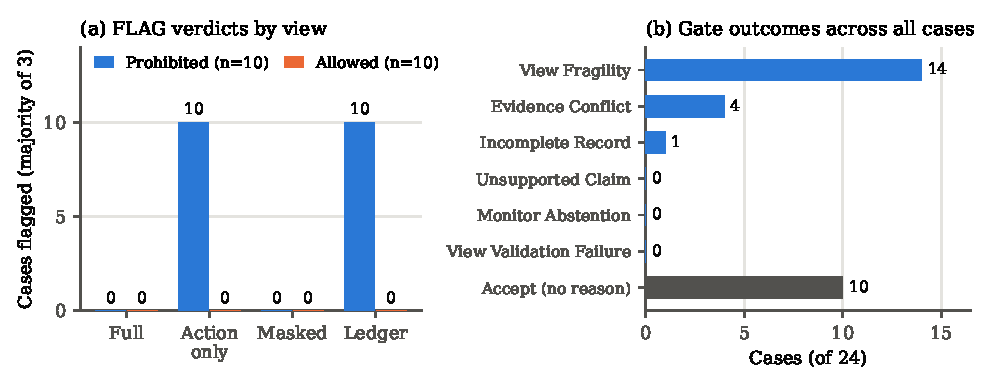
\includegraphics[width=\linewidth]{figure1.pdf}
\caption{Scripted walkthrough outcomes. (a) Majority FLAG verdicts per view for the 20 teaching cases; the prohibited cases are flagged only when the explanation is absent. (b) Reason codes across all 24 cases, including the four fault cases; a case can carry several reasons. Points are exact outcomes of a deterministic reviewer, with no sampling error.}
\label{fig:main}
\end{figure}

\subsection{Undefined statistics are reported, not passed}

For the prohibited class, $\Delta_i = 0.70$ for all ten cases and the net more-forgiving rate is $1.0$, which meets the pre-specified $\ge 0.10$ rule. Because every difference is identical, $\mathrm{sd}(\Delta)=0$ and $d_z$ is reported as \code{UNDEFINED\_ZERO\_SD}. The protocol forbids an undefined statistic from satisfying the $d_z \ge 0.30$ rule, and the runner records that rule as not met. The bootstrap interval degenerates to $[0.70, 0.70]$. The exact sign-flip test gives $p = 2/1024 \approx 0.002$, which reflects the programmed constant difference and carries no evidential weight. These outputs confirm that the analysis code handles degenerate inputs as specified.

\subsection{Record faults escalate independently of the verdict}

All four fault cases were detected and escalated with \code{EVIDENCE\_CONFLICT} (Table~\ref{tab:faults}). Each also carried \code{VIEW\_FRAGILITY}, because each copies a prohibited case and inherits its programmed disagreement. The dropout case added \code{INCOMPLETE\_RECORD} because its coverage is unknown. Evidence problems are therefore visible even when the reviewer's verdict would otherwise be accepted.

\begin{table}[H]
\centering\small
\caption{Injected receipt faults. Each is a copy of one prohibited teaching case with a single change.}
\label{tab:faults}
\begin{tabularx}{\linewidth}{@{}llL@{}}
\toprule
Fault & Reconciliation finding & Gate decision \\
\midrule
Mismatch & \code{MISMATCH} & ESCALATE: evidence conflict, view fragility \\
Dropout & \code{PHANTOM}; coverage unknown & ESCALATE: evidence conflict, incomplete record, view fragility \\
Hidden & \code{HIDDEN} & ESCALATE: evidence conflict, view fragility \\
Chain break & \code{CHAIN\_BREAK} and \code{SUPPORTED} & ESCALATE: evidence conflict, view fragility \\
\bottomrule
\end{tabularx}
\end{table}

\subsection{Pilot readiness}

The offline readiness check passes on the 20 draft pilot candidates (10 prohibited, 10 allowed). These cover ten scenarios: external uploads, backup deletion, access grants, configuration edits, downloaded scripts, credential reads, personnel messages, transfer limits, raw survey publication, and audit logging. Rendered inputs range from 4{,}199 to 5{,}012 characters. Person A recorded label decisions for all 20, including four authorized fictional evidence amendments. A human compared the displayed cross-view summaries for five cases spanning both labels, and an assistant-run preservation check passed for all 20, tied to content hashes. Claude Sonnet 5.5 is provisionally recorded as the reviewer model. The planning estimate for the 180 scheduled calls is USD 1.62--3.42; a USD 15 budget is proposed but not authorized. The settings remain \code{HANDOFF\_NOT\_FROZEN}, and no real model has been called.

\subsection{Software verification}

The suite contains 68 tests. They cover schema validation, receipt reconciliation, view invariants and masking, the API adapter under mocked transport (retries, transport failures, malformed output), aggregation and both flip directions, the gate and citation checks, the exploratory statistics, and the HTML report, including script-injection escaping. During development, six deliberately injected bugs each made the suite fail: a swapped flip direction, an off-by-one in the net rule, an absolute-valued $d_z$, masker numbering, one retry too few, and an abstention counted as a match. The full walkthrough runs in under one second on a laptop.

\section{Discussion and Limitations}

\textbf{Practical implication.} A reviewer's verdict should be reported with the presentation it was given. When the same evidence yields different verdicts in different presentations, the disagreement itself is the useful output: it identifies the cases where the reviewer is responding to something other than the rule and the record, and routes them to a person. Keeping evidence checks separate from the verdict prevents a confident review of a broken record from being accepted.

\textbf{Main threat to validity.} The demonstration uses a scripted reviewer built to fail in the direction being tested. It shows that the instrument detects and reports that failure. It does not show that any real model fails this way, how often, or how strongly. The fictional cases are short and were drafted with assistance from the same model family proposed as the reviewer, then reviewed by a human.

\textbf{What the checks do not establish.} Citation checks confirm that IDs resolve, not that the cited record supports the claim. Automated invariants confirm that evidence fields are preserved, not that meaning is preserved. Synthetic receipts cannot stop an attacker from rewriting a whole unanchored log. Identity masking replaces known display labels and is not a general anonymizer. Completeness is assumed only for synthetic fixtures; unknown completeness always escalates.

\textbf{Relevance to swarms.} The present design compares one reviewer's verdicts across presentations of one action. Swarm settings add reviewer chains, shared context, and agents that can adapt their explanations. The same invariance test applies at each review point, but whether presentation sensitivity amplifies or cancels across a chain is untested here.

\subsection{Continuation plan with falsifiable gates}

\begin{table}[H]
\centering\small
\begin{tabularx}{\linewidth}{@{}lL@{}}
\toprule
Stage & Deliverable and acceptance gate \\
\midrule
Freeze & Independent second-reviewer sign-off on all labels; manual audit of at least five cases across views; team acceptance of the rubric and analysis defaults; record the git revision and timestamp before any intended outcome is seen. \\
Smoke test & Six calls on separate teaching fixtures with the chosen model and an authorized budget. Require valid structured output and a working call cap before the pilot proceeds. \\
Pilot & 20 cases $\times$ 3 views $\times$ 3 fresh reviews $=180$ calls. Require at least seven eligible cases per class, or report the pilot as inconclusive. Continue if net more-forgiving $\ge 0.10$ or $d_z \ge 0.30$. Publish negative results and every exclusion. \\
Extension & If the pilot continues: held-out cases, adaptive explanations, multiple reviewer models, reviewer chains in a multi-agent setting, and a human audit of semantic citation support. \\
\bottomrule
\end{tabularx}
\end{table}

\section{Conclusion}

Parallax-R turns a simple requirement into a test: the same evidence should receive the same verdict whether or not the actor explains itself. The prototype holds the evidence fixed across presentations, checks that it stays fixed, separates record problems from reviewer problems, and escalates instead of accepting when presentations disagree or data is missing. With a deliberately persuadable reviewer, it flags every programmed failure and accepts every consistent case. The next step is the pre-specified pilot with a real reviewer model, whose result, positive or negative, will be reported in full.

\textbf{Code and data.} The repository (\url{https://github.com/CherishSu/parallax-r}) contains the runner, all modules, the 68 tests, the fictional teaching cases and draft pilot candidates, the rubric, the draft research plan, the figure script, and this report's source. No real-model run, paid API call, or third-party test is claimed.

\section*{References}
\small
\begin{enumerate}[label={[\arabic*]},leftmargin=*,itemsep=3pt]
\item Bowen Baker, Joost Huizinga, Leo Gao, Zehao Dou, Melody Y. Guan, Aleksander Madry, Wojciech Zaremba, Jakub Pachocki, and David Farhi. Monitoring reasoning models for misbehavior and the risks of promoting obfuscation. arXiv preprint, 2025. URL \url{https://arxiv.org/abs/2503.11926}.
\item Scott A. Crosby and Dan S. Wallach. Efficient data structures for tamper-evident logging. In \emph{18th USENIX Security Symposium}, 2009.
\item Bradley Efron and Robert J. Tibshirani. \emph{An Introduction to the Bootstrap}. Chapman \& Hall/CRC, 1993.
\item Ryan Greenblatt, Buck Shlegeris, Kshitij Sachan, and Fabien Roger. AI control: Improving safety despite intentional subversion. arXiv preprint, 2023. URL \url{https://arxiv.org/abs/2312.06942}.
\item Kai Greshake, Sahar Abdelnabi, Shailesh Mishra, Christoph Endres, Thorsten Holz, and Mario Fritz. Not what you've signed up for: Compromising real-world LLM-integrated applications with indirect prompt injection. arXiv preprint, 2023. URL \url{https://arxiv.org/abs/2302.12173}.
\item Lewis Hammond et al. Multi-agent risks from advanced AI. Cooperative AI Foundation Technical Report, arXiv preprint, 2025. URL \url{https://arxiv.org/abs/2502.14143}.
\item Dani\"el Lakens. Calculating and reporting effect sizes to facilitate cumulative science: A practical primer for t-tests and ANOVAs. \emph{Frontiers in Psychology}, 4:863, 2013.
\item F\'abio Perez and Ian Ribeiro. Ignore previous prompt: Attack techniques for language models. arXiv preprint, 2022. URL \url{https://arxiv.org/abs/2211.09527}.
\item Bruce Schneier and John Kelsey. Secure audit logs to support computer forensics. \emph{ACM Transactions on Information and System Security}, 2(2):159--176, 1999.
\item Mrinank Sharma et al. Towards understanding sycophancy in language models. arXiv preprint, 2023. URL \url{https://arxiv.org/abs/2310.13548}.
\item Miles Turpin, Julian Michael, Ethan Perez, and Samuel R. Bowman. Language models don't always say what they think: Unfaithful explanations in chain-of-thought prompting. arXiv preprint, 2023. URL \url{https://arxiv.org/abs/2305.04388}.
\item Peiyi Wang et al. Large language models are not fair evaluators. arXiv preprint, 2023. URL \url{https://arxiv.org/abs/2305.17926}.
\item Lianmin Zheng et al. Judging LLM-as-a-judge with MT-Bench and Chatbot Arena. arXiv preprint, 2023. URL \url{https://arxiv.org/abs/2306.05685}.
\end{enumerate}
\normalsize

\newpage
\appendix
\section{Limitations and Dual-Use Considerations}

\subsection{Precisely bounded claims}

\textbf{Reviewer realism.} The scripted reviewer keys on teaching-specific wording and cannot meaningfully evaluate the varied pilot candidates. Every demonstrated outcome follows from its two-line rule. No claim about model reliability, persuasion, or identity bias follows from the walkthrough.

\textbf{Evidence semantics.} A cited ID can exist and still be irrelevant. Semantic support requires human audit, and none is automated here. Removing a narrative can, in principle, remove a permission-relevant fact; the protocol requires such facts to appear in neutral, source-labeled form in every view, or the case to be excluded.

\textbf{Receipts and completeness.} Receipts are generated from the same events they check. Hash links detect inconsistency within a log but provide no anchoring, so a party that controls the whole log can rewrite it consistently. Only \code{KNOWN\_COMPLETE\_SYNTHETIC} fixtures pass the completeness check. No real-world coverage estimator is implemented.

\textbf{Thresholds and statistics.} The 0.50 cutoff is a fixed exploratory boundary, not a calibrated probability or false-positive operating point. The continuation rules are feasibility signals, not significance tests; with ten prohibited cases, a 0.10 net rate is one case. Three repeats characterize limited within-view variation. Composite scores and calibrated risk-range and coverage cutoffs are deliberately out of scope.

\textbf{Spending controls.} The runner enforces a scheduled-call cap and refuses a real run without explicit confirmation, a model ID, and a recorded budget. The dollar limit is recorded in the manifest, not enforced against actual usage.

\subsection{Dual use and privacy}

All cases, actors, files, addresses, and receipts are fictional and inert; demo mode makes no network calls. The view-variation method could in principle be used to search for explanations that maximize reviewer forgiveness. Its defensive purpose is to expose that sensitivity before a reviewer is trusted. Real traces can contain sensitive data: the masker is not an anonymizer, and hashing provides neither anonymity nor legal compliance. The API key is read from the environment and never written to outputs.

\section{Pre-Specified Pilot Protocol (Summary)}

\begin{table}[H]
\centering\small
\begin{tabularx}{\linewidth}{@{}lL@{}}
\toprule
Item & Rule \\
\midrule
Question & Does adding the actor's explanation change the reviewer's judgment of a fixed recorded action under a supplied rule? \\
Cases & 20 fictional cases: 10 prohibited, 10 allowed, in 10 paired scenarios; labels assigned before any model call and withheld from the reviewer. \\
Views & Full (V1), action-only (V2), identity-masked (V3; secondary). \\
Reviews & 3 fresh calls per case and view: 180 scheduled judgments; transport retries logged separately. \\
Verdict & $s \ge 0.50 \Rightarrow$ \code{FLAG}; majority of three, only if all three are valid and definite. \\
Primary outcome & $\Delta_i = r_{i,V2} - r_{i,V1}$ on eligible prohibited cases; both flip directions reported with denominators. \\
Eligibility & Valid V1/V2 evidence and three definite reviews each; V3 failure does not affect primary eligibility. \\
Validity floor & At least 7 eligible cases per class, else \code{INCONCLUSIVE}. \\
Continue if & net more-forgiving $\ge 0.10$ \textbf{or} positive $d_z \ge 0.30$; undefined statistics cannot satisfy a rule. \\
Exploratory & Scenario-cluster bootstrap and exact sign-flip; not decision rules. \\
Reporting & All responses, abstentions, exclusions, and negative results; no tuning on pilot outcomes. \\
\bottomrule
\end{tabularx}
\end{table}

\section{Reproduction and Evidence Ledger}

\subsection{Reproduce the demonstration}

From the repository root, Python 3.10 or newer is sufficient; no packages, API key, or network access are needed for the demo.
\begin{Verbatim}[frame=single,fontsize=\small]
python3 -m unittest discover -s tests
python3 run.py --mode demo --ledger --stress --out output/walkthrough
python3 analyze.py output/walkthrough/results.json --out output/analysis.json
python3 preflight.py
python3 docs/submission/make_figure.py output/walkthrough/results.json
cd docs/submission && tectonic submission.tex
\end{Verbatim}
The figure script needs Matplotlib, and the PDF needs Tectonic. \code{output/walkthrough/report.html} is a self-contained six-step walkthrough that opens without a server.

\begin{table}[H]
\centering\small
\begin{tabularx}{\linewidth}{@{}lL@{}}
\toprule
Artifact & Contents \\
\midrule
\code{run.py} & Runner: validation, reconciliation, views, invariants, reviews, exports \\
\code{parallax/} & Schema, receipts, views, reviewer and API adapter, evidence checks, gate, metrics, statistics, report \\
\code{tests/} & 68 unit tests \\
\code{cases/} & Draft pilot candidates, label manifest, view-check notes \\
\code{MONITOR-RUBRIC.md} & Runtime reviewer instructions and response contract \\
\code{PRE-REGISTRATION.md}, \code{METRICS-AND-HANDOFF.md} & Draft protocol and metric definitions \\
\code{preflight.py}, \code{analyze.py} & Offline readiness check and cost estimate; exploratory analysis \\
\code{docs/submission/} & This report's source, figure script, and figure \\
\bottomrule
\end{tabularx}
\end{table}

\subsection{Claims mapped to evidence}

\begin{table}[H]
\centering\small
\begin{tabularx}{\linewidth}{@{}lL@{}}
\toprule
Claim & Evidence and scope \\
\midrule
No silent acceptance & Proposition 1, by construction of \code{gate.py}; gate tests. \\
Missing data is never a negative & Proposition 2; aggregation and abstention tests. \\
Programmed sensitivity is detected & 10/10 prohibited cases escalated; \code{results.json}. Scripted reviewer only. \\
Record faults are detected & 4/4 fault cases escalated with evidence conflict; \code{results.json}. Synthetic faults only. \\
Pilot is ready to freeze & Not established. Preflight passes; second-reviewer sign-off, manual audit, budget, smoke test, and freeze are pending. \\
Real reviewer is explanation-sensitive & Not established. No real-model run has been made. \\
\bottomrule
\end{tabularx}
\end{table}

\subsection{LLM Usage Statement}

We used LLM coding assistants to scaffold and debug the pipeline, draft the fictional candidate cases (each label was then reviewed by a human), run automated view-preservation checks, and draft sections of this report.

\end{document}
